%% Outline
% 1. Navigation is important problem
% 1.5 Traditionally addressed by mapping during exploration and path
%      planning during exploitation.
% 2. End to end learning algorithms have shown promise to take over
%      mapping and path
% 3. We do not know how these algorithms work. There has been work in computer vision that shows the learning on neural network based methods can be learning totally different kind of patterns from what we would expect.
% 4.1 We find that it is not remembering the map it is being trained on
% 4.2 We find that no path planning is  happening only, memorizing and regeneration of the sequence of steps. However, it is not 

% 1. Navigation is important problem
% 1.5 Traditionally addressed by mapping during exploration and path
%      planning during exploitation.
Navigation remains a fundamental problem in mobile robotics and artificial intelligence (\cite{SmChIJRR1986,ElCOMPUTER1980}).
The problem is classically addressed by separating the task of navigation into two steps, exploration and exploitation. 
In the exploration stage, the environment is represented as some kind of \emph{map}. 
In the exploitation stage, the map is used to \emph{plan a path} to a given destination based on some optimality criterion. 
% VD: SLAM is just the exploration part. I think we should avoid introducing SLAM here.
% VD: why do we need to mention autonomous driving industry
 %This classical approach, traditionally called SLAM (Simultaneous Localization and Mapping), constitutes an entire subfield of robotics whose successes include the birthing of the autonomous driving industry. 
% SLAM however, possesses its own limitations.
This classical approach has been quite successful in navigation using a variety of sensors.
However, navigation in general unstructured environments, especially with texture-less \cite{YaSoKaIROS2016}, transparent and reflective surfaces \cite{lai2011large}, remains a challenge.
% VD: ``subtly different'' Too generic of a claim
%Algorithms, especially those centered in vision, lack performance invariance often failing to extend results to environments that are subtly different from the ones they were trained on.
%As a simple example, state-of-the-art monucular SLAM methods fail when confronted with textureless environments.
% Moreover, in many application the mapping in full metric detail is unnecessary, which has prompted researchers to non-metric maps like topological maps \cite{beeson2010factoring}. However, with the decisions regarding 
% Furthermore, the decision about the required mapping details depends upon the end task of path planning, hence requires difficult decisions about the encoding of mapping data structures.


Recently, end-to-end navigation methods---which attempt to  
solve the navigation problem without breaking it down into separate parts of mapping and path-planning---have gained traction.
%
% 2. End to end learning algorithms have shown promise to take over
%      mapping and path-planning
With the recent advances in Deep Reinforcement Learning (DRL), these end-to-end navigation methods, such as \cite{MnBaMiICML2016,SiHuMaNATURE2016,LePaKrISER2017,MiPaViICLR2017,OhChSiICML2016}, forego decisions about the details that are required in the intermediate step of mapping.
The potential for simpler yet more capable methods is rich; for example, the resulting trained agents can potentially optimize the amount of map information required for navigation tasks.
One such algorithm by \cite{MiPaViICLR2017} has shown promise in exploring and finding the goal efficiently within complex environments. Notably, this is done using only monocular first-person views.
%Of significance is the fact that these agents upon finding the goal within a previously seen environment, are able to navigate to it faster in subsquent explorations implying that agents are able to learn to exploit map structures in the execution of learned navigational tasks. 

\begin{figure}
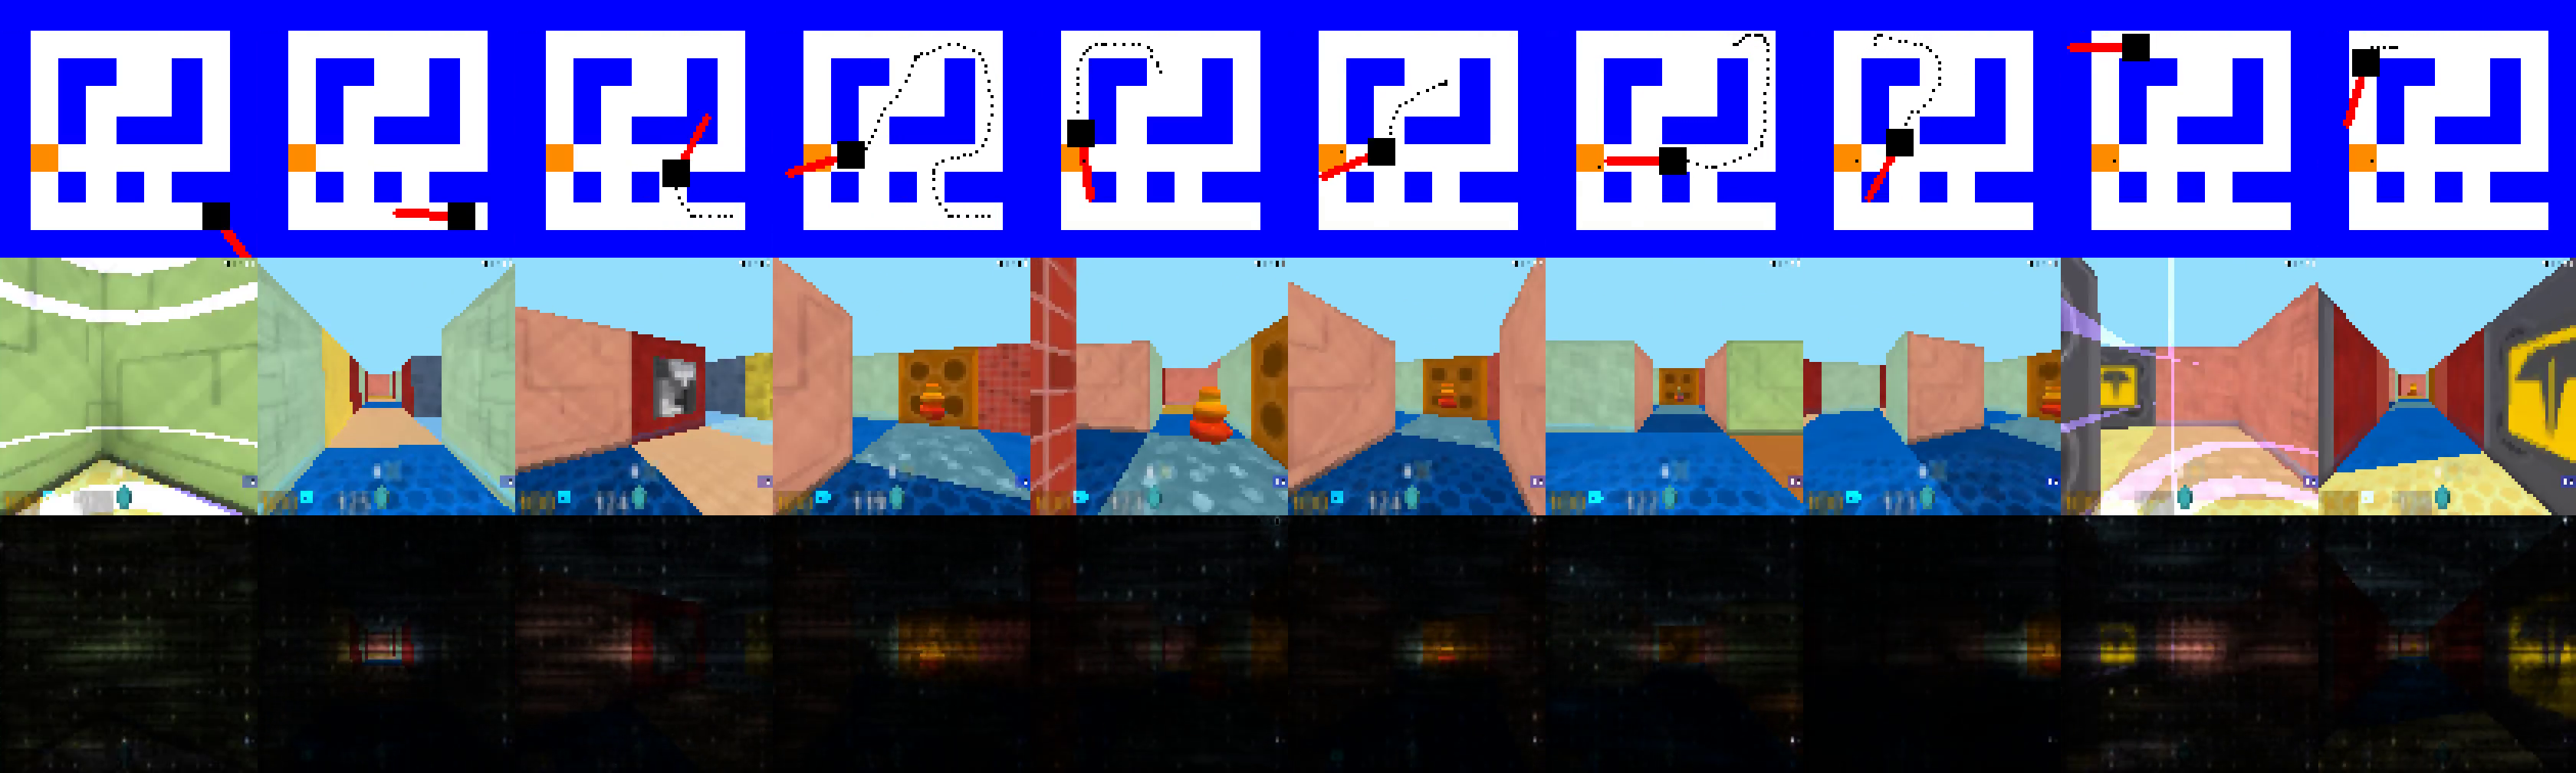
\includegraphics[width=\textwidth,trim=0 336pt 0 0,clip]{./exp-results/training-09x09-0127-on-0127.png}%
\caption{
Snapshots of the path taken by the agent while evaluating the model trained on the same random map with random goal and random spawn.
% JJC: TODO: make sure that you communicate that the top view is not available to the algorithm.
The first row shows the top view of the robot moving through the maze with the goal location marked orange, the agent marked black and the agent's orientation marked red. The second row shows the first person view, which, besides reward, is the only input available to the agent.}
\label{fig:training-qualitative}
\end{figure}

% 3. We do not know how these algorithms work. There has been work in computer vision that shows the learning on neural network based methods can be learning totally different kind of patterns from what we would expect.
Despite such potential advances, DRL-based navigation remains a relatively unexplored field with its own limitations. 
The black-box nature of these methods make them difficult to study, and the patterns captured by the methods are not well understood. 
% VD: This is not the limitation of DRL algorithms
%Their exists no comprehensive set of experiments that answer how and when these algorithms perform well and how their performance differs based on variations in the training and testing conditions. 
% VD: This is a detail and is repeated in next paragraphs
% It is also unknown how well these algorithms generalize especially to previously unseen worlds.
Recent work analyzing neural networks has shown that deep learning-based object detection methods can be easily fooled by introducing noise that is imperceptible to humans (\cite{NgYoClCVPR2015}); this motivates why it is particularly important to analyze DRL methods across a wide variety of experiments: we need to understand their strengths and limitations.

% 4.1 We find that it is not remembering the map it is being trained on
% 4.2 We find that no path planning is  happening only, memorizing and regeneration of the sequence of steps. However, it is not 

% Prior setup
% JJC: TODO: Generalize to multiple fields
In this work, we develop a better understanding of recent DRL-based methods. In particular, we thoroughly explore and analyze the state-of-the-art \cite{MiPaViICLR2017} methods across hundreds of maps with increasing difficulty levels. 
% VD: Cutting down unncessary sentences
% VD: No need to tell the license and name of the environment
%Our setup is similar, utilizing the same simulation environment, Deepmind Lab \cite{BeLeTeARXIV2016}.
We set up the environment as a randomly generated map, as shown in Fig~\ref{fig:training-qualitative}, with an agent and a goal.
% VD: Defining the objective in terms of reward is wrong because designing rewards is a part of reinforcement learning not the problem statement.
The agent is provided only with the first-person view and is tasked to find the goal as many times as possible within a fixed amount of time, re-spawning its location each time it reaches the goal. 
We train and evaluate the algorithms with increasing difficulty.
In the easiest stage, we keep the goal location, spawn location and map constant over the training and testing.
We call this set up \emph{static goal, static spawn, and static map}.
To increase the difficulty, we incrementally randomize the spawn locations, goal locations and map structures until all three are random.
We discuss the design of experiments in Section~\ref{sec:navtasks} in more detail.
%We randomly genereate our mazes wherein the agent and goal are both statically and randomly spawned across experiments. 

\cite{MiPaViICLR2017} do train and test their algorithms with randomized goals and spawns and show that their algorithm is able to exploit the knowledge of the goal location at evaluation time to maximize reward.
However, following training and testing on constant map structures, this state-of-the-art result is shown to be successful on only one map, which brings into question the repeatability of the results.
It is also unclear whether these results generalize to unseen maps.

Although disjoint training and testing sets are standard practice in machine learning, to the best of our knowledge, we are the first to evaluate any DRL-based navigation method on maps with unseen structures.
We expand on the analysis in \cite{MiPaViICLR2017} to address its limitations and ask whether DRL-based algorithms such as \NavAiiiCDiDiiL{} perform any mapping followed by shortest path planning.
Our experiments show no evidence of mapping in cases where algorithms are evaluated on unseen maps and no evidence of optimal path planning, even when the map is constant and only the goal is randomized.

To better understand navigation, we compute attention-maps for models to show which portions of the input image are being used.
We find that the models discard most of the image information, focusing attention on a small band in the middle of the image except around junctions, in which case the attention is distributed evenly throughout the image.

These findings result from training and testing on multiple maps that were randomly selected from a set of 1100 randomly generated maps.
We provide experimental results on ten randomly selected maps and a testing set of 100 unseen maps to ensure results are independent of map choice.
We will make our code and data available following the blind review process.

% Explained earlier
% % Systematic experiments
% To address this lacks of information about these agent's navigational abilities, we systematically expand upon \cite{MiPaViICLR2017}'s analysis by evaluate these agents and  metrics on a comprehensive set of randomly generated maps with differing training and testing conditions of increasing complexity. 
% In particular, we move from deterministic setups wherein the agents are trained on environments containing fixed spawn points, fixed goal locations and coincident training/testing maps to  much more complex cases involving random spawn points, random goal locations and diverged training and testing sets. 
% In particular, we quantitavely evaluate our trained models to test their map-exploitation abilitiesacross these differing setups and observe agents are unable to transfer this ability to the unseen worlds.
% Instead we observe that the agent's preferred path to the goal is just as an artifact of its initialized location and rotation and hypothesize that the agents are learning a correspondence between local sequences of frames and actions that lead to the goal.

% More contributions


